% \textbf{\underline{OZ 6 - Magnetische inductie en de wet van Faraday - Oefening 2:}}
% \vspace{0.5cm}

% Twee parallele geleidende rails met verwaarloosbare wrijving liggen 10,0 cm van elkaar en zijn verbonden via een weerstand van $ 5,00 \ \Omega $. Twee geleidende staven met weerstanden $ 10,0 \ \Omega $ en $ 15,0 \ \Omega $ worden aangebracht op de rails zoals in Figuur 6.2. De staven worden weggetrokken van de $ 5,00 \ \Omega $ weerstand met constante snelheden 4,00 m/s en 2,00 m/s. Een uniform magneetveld van 0,0100 T wordt aangelegd loodrecht op het vlak van de rails. Bepaal de stroom die door de $ 5,00 \ \Omega $ weerstand gaat lopen.

% \begin{figure}[H]
%     \centering
%     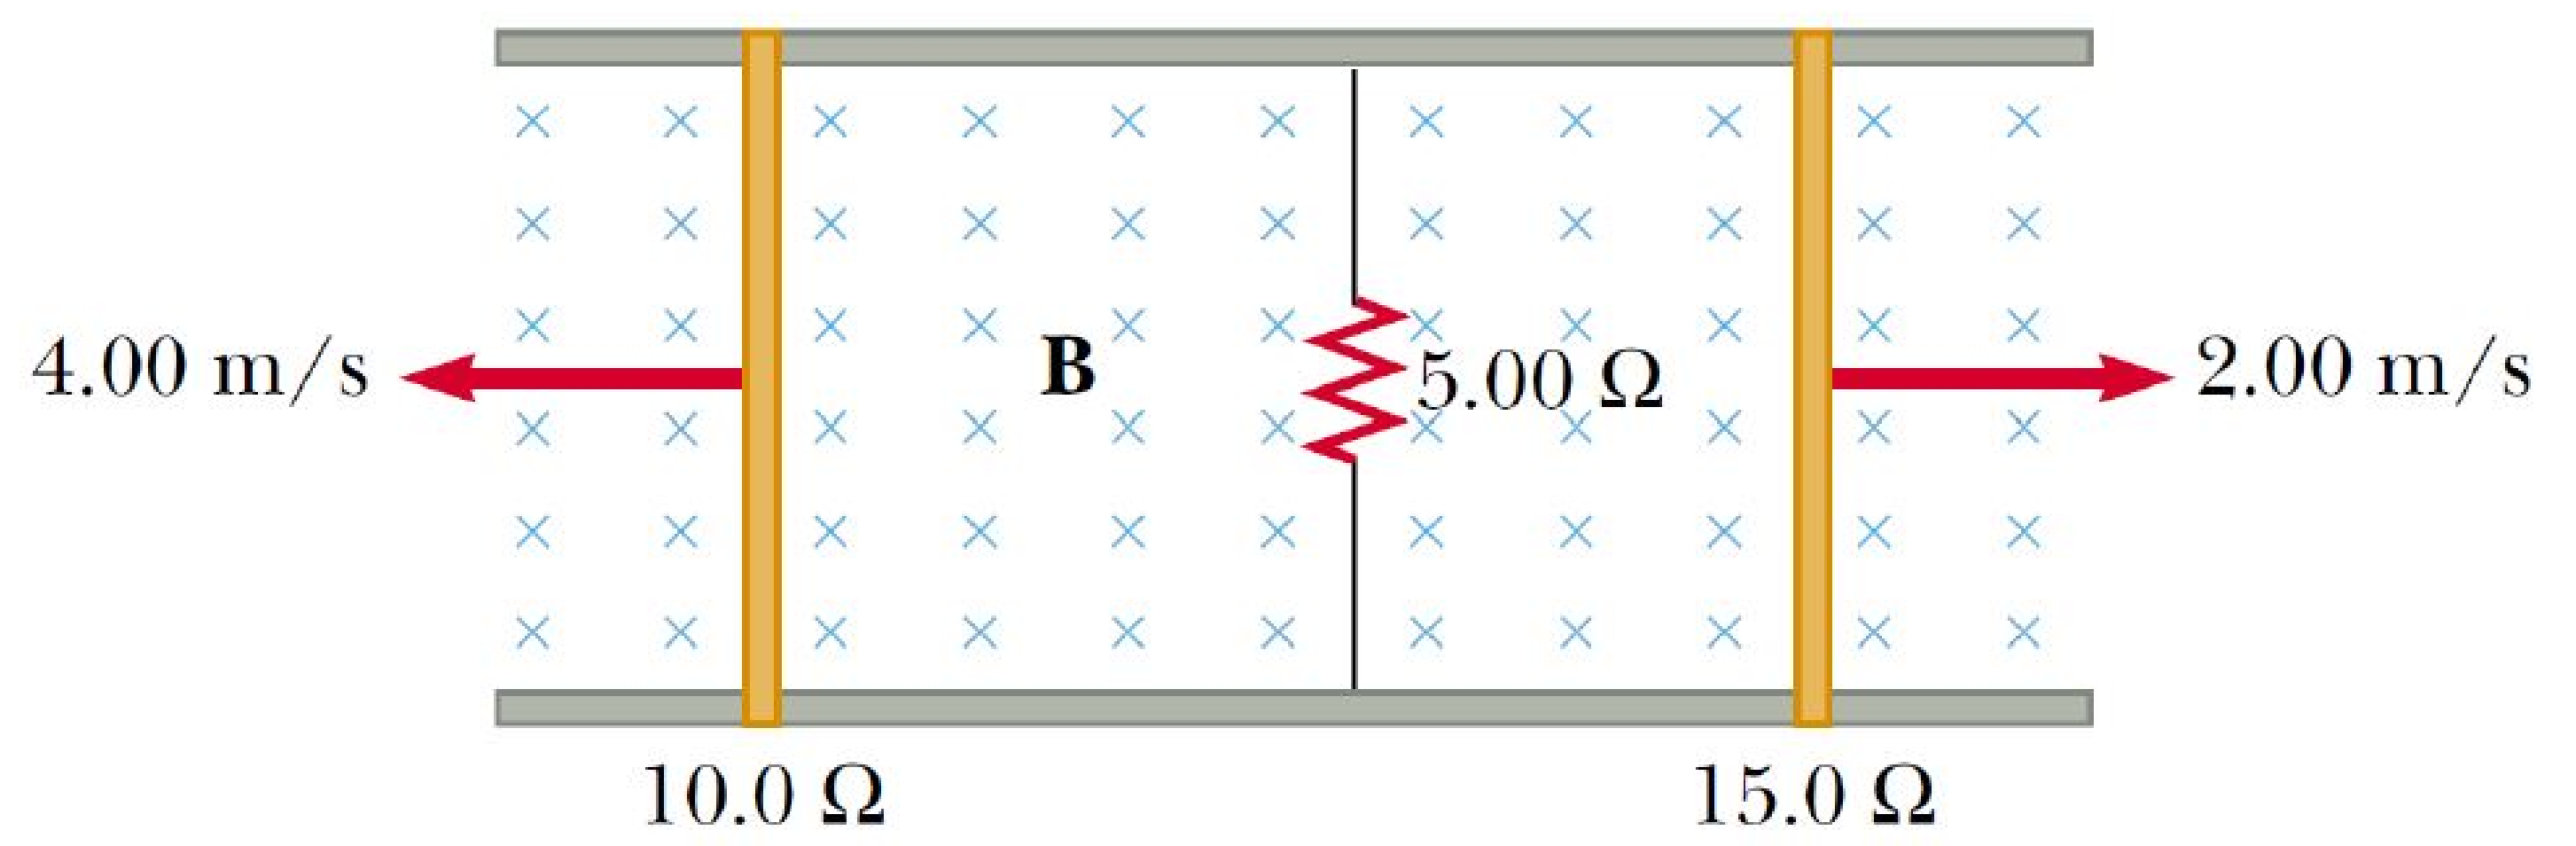
\includegraphics[width=9cm]{oz06/resources/oef-2-opgave.png}
    
%     \textbf{Figuur 6.2}
% \end{figure}

% \begin{description}[labelwidth=1.5cm, leftmargin=!]
%     \item[Geg. :]   $ l = 10,0 $ cm; $ R = 5,00 \ \Omega $; $ R_1 = 10,00 \ \Omega $; $ R_2 = 15,00 \ \Omega $; $ v_1 = 4,00 $ m/s; $ v_2 = 2,00 $ m/s; $ B = 0,0100 $ T;
% \end{description}

% \begin{figure}[H]
%     \centering
%     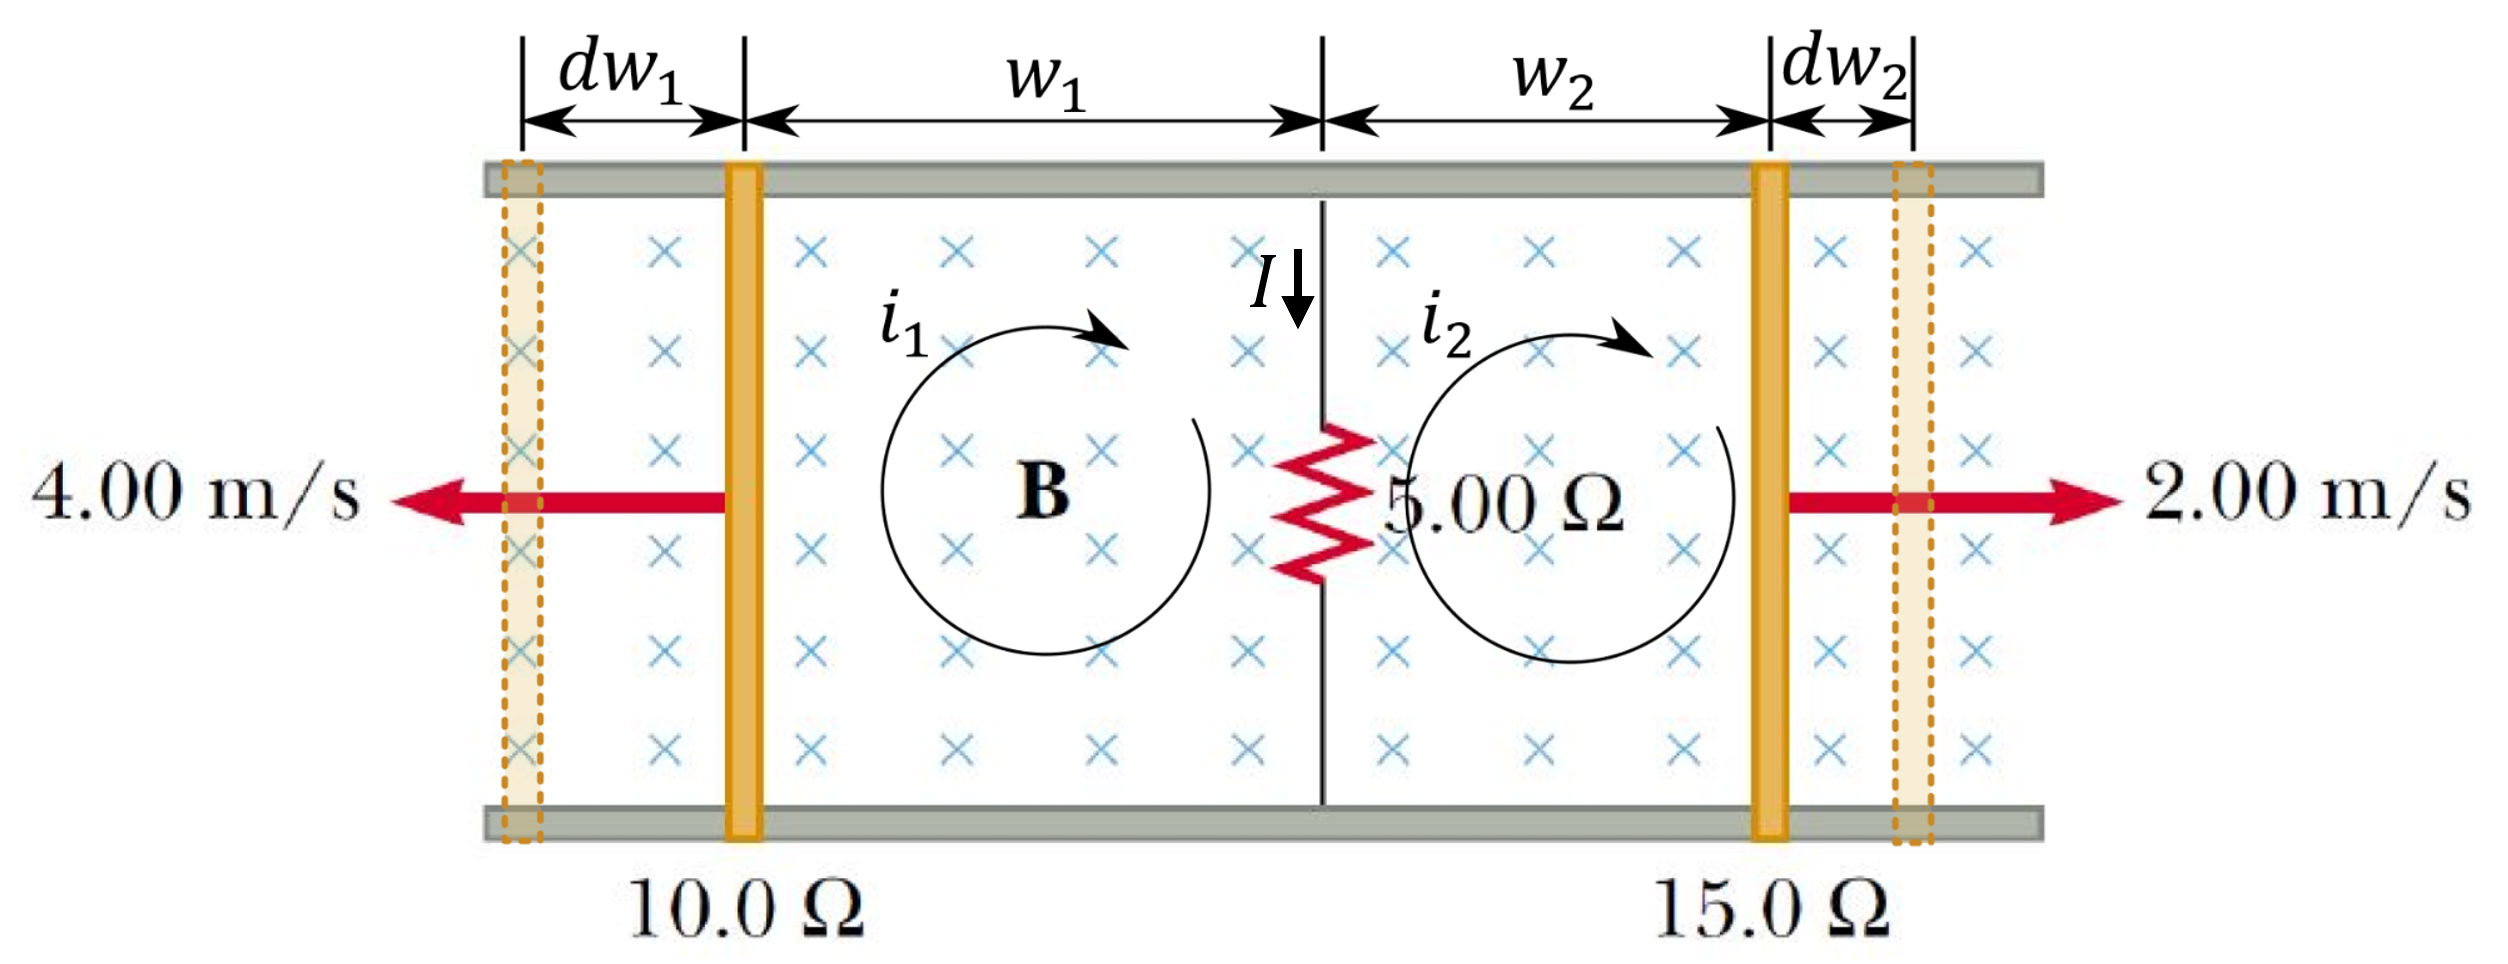
\includegraphics[width=9cm]{oz06/resources/oef-2-schets.png}
    
%     \textbf{Schets 6.2}
% \end{figure}

% \begin{description}[labelwidth=1.5cm, leftmargin=!]
%     \item[Gevr. :]  $ I $;
%     \item[Opl. :]   $ A_1 = l \cdot \left( w_1 + dw_1 \right) = l \cdot \left( w_1 + v_1 t \right) $
    
%                     $ \Phi_1 = \int{ \vec{B} \cdot d\vec{A_1}} 
%                     = B \cdot A_1 
%                     = B \cdot l \cdot \left( w_1 + v_1 t \right) $
                    
%                     \hspace{-0.57cm} $ \Rightarrow 
%                     \dfrac{d\Phi_1}{dt} = B \cdot l \cdot v_1 $
                    
%                     $ \varepsilon_1 = -\dfrac{d\Phi_1}{dt} = -B \cdot l \cdot v_1 $
                    
%                     $ i_1 = \dfrac{\varepsilon_1}{R + R_1} = \dfrac{-B \cdot l \cdot v_1}{R + R_1} = \dfrac{-0,0100 \cdot 10,0 \cdot 10^{-2} \cdot 4,00}{5,00 + 10,00} = -0,00026667 $ A
                    
%                     \vspace{0.5cm}
                    
%                     $ A_2 = l \cdot \left( w_2 + dw_2 \right) = l \cdot \left( w_2 + v_2 t \right) $
    
%                     $ \Phi_2 = \int{ \vec{B} \cdot d\vec{A_2}} 
%                     = B \cdot A_2 
%                     = B \cdot l \cdot \left( w_2 + v_2 t \right) $
                    
%                     \hspace{-0.57cm} $ \Rightarrow 
%                     \dfrac{d\Phi_2}{dt} = B \cdot l \cdot v_2 $
                    
%                     $ \varepsilon_2 = -\dfrac{d\Phi_2}{dt} = -B \cdot l \cdot v_2 $
                    
%                     $ i_2 = \dfrac{\varepsilon_2}{R + R_2} = \dfrac{-B \cdot l \cdot v_1}{R + R_2} = \dfrac{-0,0100 \cdot 10,0 \cdot 10^{-2} \cdot 2,00}{5,00 + 15,00} = -0,0001 $ A
                    
%                     \vspace{0.5cm}
                    
%                     \textcolor{orange}{$ I = i_1 - i_2 
%                     = -0,00026667 - (-0,0001) 
%                     = -0,00016667 $ A $ 
%                     \approx -0,167 $ mA}
                    
%                     \textcolor{orange}{Resultaat verschilt van gekregen uitkomst (0,145 mA)}
% \\\\\\\\
% \item[Opl. 2 :] (Oplossing van Serway 6E Chapter 31 Problem 31)

% Name the currents as shown in the diagram:
% $$
% \begin{aligned}
% & \text{Left loop:} & +B d v_2-I_2 R_2-I_1 R_1=0 \\
% & \text{Right loop:} & +B d v_3-I_3 R_3+I_1 R_1=0 \\
% & \text{At the junction:} & I_2=I_1+I_3 \\
% & \text{Then,} & B d v_2-I_1 R_2-I_3 R_2-I_1 R_1=0
% \end{aligned}
% $$
% $I_3=\frac{B d v_3}{R_3}+\frac{I_1 R_1}{R_3}$.
% $$
% \begin{aligned}
% & \text{So,} & B d v_2-I_1\left(R_1+R_2\right)-\frac{B d v_3 R_2}{R_3}-\frac{I_1 R_1 R_2}{R_3}=0
% \end{aligned}
% $$
% $I_1=B d\left(\frac{v_2 R_3-v_3 R_2}{R_1 R_2+R_1 R_3+R_2 R_3}\right)$ upward
% \\
% $I_1=(0.0100 \mathrm{~T})(0.100 \mathrm{~m})\left[\frac{(4.00 \mathrm{~m} / \mathrm{s})(15.0 \Omega)-(2.00 \mathrm{~m} / \mathrm{s})(10.0 \Omega)}{(5.00 \Omega)(10.0 \Omega)+(5.00 \Omega)(15.0 \Omega)+(10.0 \Omega)(15.0 \Omega)}\right]=145 \mu \mathrm{A}$ upward.
                    
% \end{description}

% \vspace{1cm}